\documentclass[preview]{standalone}

\usepackage{amsmath}
\usepackage{amssymb}
\usepackage{stellar}
\usepackage{bettelini}
\usepackage{tikz}
\usepackage{wrapfig}
\usepackage{definitions}

\begin{document}

\id{envelope-curves}
\genpage

\section{Envelope curves}

\begin{snippetdefinition}{envelope-definition}{Envelope}
    A differentiable curve \(\sigma \colon I \fromto \realnumbers^2\)
    with non-zero derivative
    is called the \emph{envelope} of the family of planar curves
    \[
        C_t = \{(x,y) \suchthat F(t, x,y) = 0\}
    \]
    if \(\sigma\) is tangent to \(C_t\) at \(\sigma(t)\)
    for every \(t\).
\end{snippetdefinition}

\begin{snippetproposition}{envelope-curve-equation}{Envelope curve equation}
    If \(\sigma(t) = (x(t), y(t))\) is the envelope of \(F(t,x,y)\),
    then the points \((t,x(t), y(t))\) are solutions to the system 
    \[
        \begin{cases}
            F(t,x(t), y(t)) = 0 \\
            F_t(t, x(t), y(t)) = 0
        \end{cases}
    \]
\end{snippetproposition}

\begin{snippetproof}{envelope-curve-equation-proof}{envelope-curve-equation}{Envelope curve equation}
    From the definition of envelope it follows that
    \[
        F(t, x(t), y(t)) = 0
    \]
    Subsequently, the tangent condition tells us that
    \begin{align*}
        0 &= \langle \gradient F(t,x(t), y(t)), \sigma'(t) \rangle \\
        0 &= \frac{\partial F}{\partial x}(t, x(t), y(t))x'(t) + \frac{\partial F}{\partial y}(t, x(t), y(t))y'(t)
    \end{align*}
    which is orthogonality to the gradient.
    By taking the total derivative of the first equation with respect to \(t\), we find
    \begin{align*}
        0 &= \frac{d}{dt} F(t,x(t),y(t)) \\
        &= \frac{\partial F}{\partial t}(t, x(t), y(t))
        + \frac{\partial F}{\partial x}(t, x(t), y(t))x'(t)
        + \frac{\partial F}{\partial y}(t, x(t), y(t))y'(t)
    \end{align*}
    Thus, putting the two expressions together, the two partial derivative terms cancel out, leaving
    the condition of the thesis.
\end{snippetproof}

\begin{snippetexample}{envelope-curve-example1}{Envelope}
    \begin{wrapfigure}{r}{6cm}
        \begin{center}
            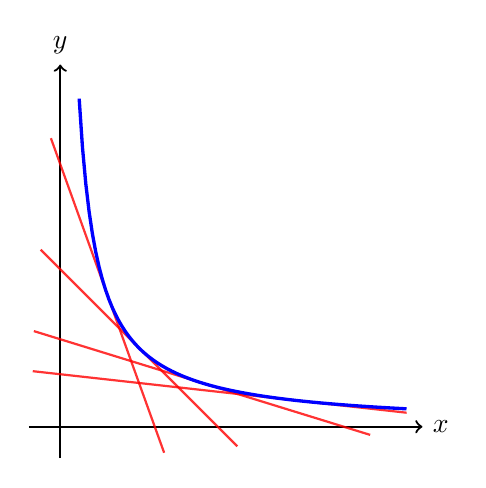
\begin{tikzpicture}[scale=2]
                \draw[->, thick] (-0.2, 0) -- (2.3, 0) node[right] {$x$};
                \draw[->, thick] (0, -0.2) -- (0, 2.3) node[above] {$y$};
                
                \clip (-0.2, -0.2) rectangle (2.2, 2.2);

                \foreach \t in {0.6, 1.0, 1.8, 3.0} {
                    \draw[red, opacity=0.8, thick, shorten >=-10pt, shorten <=-10pt] (0, {1/\t}) -- ({\t}, 0);
                }

                \draw[blue, very thick, domain=0.12:2.2, samples=100] plot (\x, {1/(4*\x)});
            \end{tikzpicture}
        \end{center}
    \end{wrapfigure}
    Consider the family of lines \[
        C_t = \{(x,y) \suchthat F(t, x,y) = 0\}
    \]
    with
    \[
        F(t,x,y) = y + \frac{1}{t^2}(x-t)
    \]
    i.e., the lines connecting \((t,0)\) to \((0, 1/t)\).
    To find the Cartesian equation of the envelope, we study the system
    \[
        \begin{cases}
            F(t,x(t), y(t)) = 0 \\
            F_t(t, x(t), y(t)) = 0
        \end{cases}
        \implies
        \begin{cases}
            y + \frac{1}{t^2}(x-t) = 0 \\
            \frac{1}{t^2} -\frac{2x}{t^3} = 0
        \end{cases}
    \]
    We derive \(t = 2x\) and substitute it
    to obtain \[4x^2y + x - 2x = 0\]
    Simplifying, we conclude that the Cartesian equation of the envelope is \(4xy = 1\).
    \wrapfill
\end{snippetexample}

\begin{snippetexample}{envelope-curve-example2}{The envelope curve does not always exist}
    If we consider the pencil of lines passing through a point, such as the origin, i.e., given
    by the equation \(F(t,x,y) = y - tx\), or the pencil of parallel lines
    \(F(t,x,y) = y - t\), the envelope curve cannot exist.
    The associated systems are, in the first case:
    \[
        \begin{cases}
            F(t,x(t), y(t)) = 0 \\
            F_t(t, x(t), y(t)) = 0
        \end{cases}
        \implies
        \begin{cases}
            y - tx = 0 \\
            -x = 0
        \end{cases}
    \]
    which implies that the support of the curve is a single point, thus it is not a curve.
    In the second case:
    \[
        \begin{cases}
            F(t,x(t), y(t)) = 0 \\
            F_t(t, x(t), y(t)) = 0
        \end{cases}
        \implies
        \begin{cases}
            y - t = 0 \\
            -1 = 0
        \end{cases}
    \]
    where there is no solution.
\end{snippetexample}

\begin{snippetproposition}{envelope-curve-characterization1}{}
    Let \(F(t, x,y) = 0\)
    be a family of lines.
    Then the envelope curve exists, and is non-constant, if and only if
    \(F\) does not express a pencil of lines.
\end{snippetproposition}

\begin{snippetproof}{envelope-curve-characterization1-proof}{envelope-curve-characterization1}{}
    We write \(F(t,x,y) = a(t)x + b(t)y + c(t)\)
    with \((a(t), b(t)) \neq (0,0)\) for all \(t\),
    and use the system's criterion requiring
    that it has solutions \((t,x,y)\)
    with \((x,y)\) non-constant. This requires excluding the pencils of lines.
    \todo
\end{snippetproof}

\begin{snippetproposition}{curve-as-envelope-of-its-tangents}{}
    Every regular planar curve is the envelope of its family of tangent lines.
\end{snippetproposition}

\end{document}